\section{Curse of Dimensionality}

\frame{
\frametitle{\secname}
\begin{columns}
\column{0.6\textwidth}
\begin{itemize}
\item As number of dimensions increases, it's easier for points to be further apart
\item Noisy dimensions obscure useful information
\item Ex: For a hypercube in $d$ dimensions with side length 1, furthest points are $\sqrt{d}$ away.
\item Many algos are exponential in input dimension
\begin{itemize}
\item $k$-d tree
\item Convex hull
\end{itemize}
\end{itemize}
\column{0.4\textwidth}

\begin{figure}
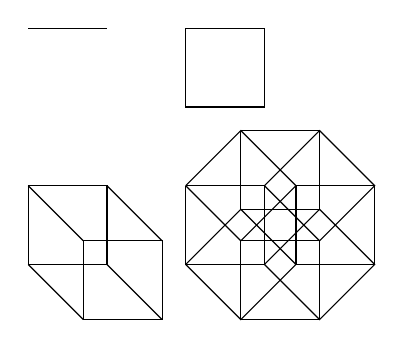
\begin{tikzpicture}
\draw (0,0) -- (1,0);

\draw (2,0) -- (2,-1) -- (3,-1) -- (3,0) -- (2,0);

\draw (0,-2) -- (0,-3) -- (1,-3) -- (1,-2) -- (0,-2);
\draw (0.7,-2.7) -- (0.7,-3.7) -- (1.7,-3.7) -- (1.7,-2.7) -- (0.7,-2.7);
\draw (0,-2) -- (0.7,-2.7);
\draw (0,-3) -- (0.7,-3.7);
\draw (1,-3) -- (1.7,-3.7);
\draw (1,-2) -- (1.7,-2.7);


\draw (2,-2) -- (2,-3) -- (3,-3) -- (3,-2) -- (2,-2);
\draw (2.7,-2.7) -- (2.7,-3.7) -- (3.7,-3.7) -- (3.7,-2.7) -- (2.7,-2.7);
\draw (2.7,-1.3) -- (2.7,-2.3) -- (3.7,-2.3) -- (3.7,-1.3) -- (2.7,-1.3);
\draw (3.4,-2) -- (3.4,-3) -- (4.4,-3) -- (4.4,-2) -- (3.4,-2);
\draw (2,-2) -- (2.7,-2.7) -- (3.4,-2) -- (2.7,-1.3) -- (2,-2);
\draw (2,-3) -- (2.7,-3.7) -- (3.4,-3) -- (2.7,-2.3) -- (2,-3);
\draw (3,-3) -- (3.7,-3.7) -- (4.4,-3) -- (3.7,-2.3) -- (3,-3);
\draw (3,-2) -- (3.7,-2.7) -- (4.4,-2) -- (3.7,-1.3) -- (3,-2);

\end{tikzpicture}
\end{figure}
\end{columns}

}